\begin{abstract}
We study regressions among 2,663 SWE-bench Verified runs that pass issue-resolution tests. Of these, 99 fail existing regression tests: a 3.72\% anomaly rate within this selected population. Our calibrated multimodal bottleneck autoencoder (CM-BAE) combines 12 structural features, MiniLM logs, and CodeBERT diffs. Autoencoder fitting uses clean runs only; labelled validation runs calibrate scores and thresholds. Issue-grouped evaluation gives average precision (AP) $0.083\pm0.028$, about $2.2\times$ prevalence. However, churn, ECOD, Isolation Forest, and XGBoost score higher. Variance equalization underperforms raw fusion. At the selected cost-based threshold, the 83.3\% false-positive rate prevents a deployment-readiness claim. The contribution is an auditable rare-regression task and an evaluation of the limits of multimodal reconstruction.
\end{abstract}

\section{Introduction}
Autonomous coding agents produce candidate repairs for real repository issues~\citep{yang2024sweagent,jimenez2024swebench}. Passing the target issue's tests is useful evidence, but does not establish that previously working behavior remains intact. We study the narrower task of screening regressions among apparently successful repairs.

An earlier project formulation treated unresolved issues as anomalies although failures comprised 81\% of its sample. That supports failure screening, but does not demonstrate rare-event detection. Here we change the population and target: candidates pass all recorded FAIL\_TO\_PASS (F2P) tests; anomalies then fail at least one PASS\_TO\_PASS (P2P) test.

This yields 2,564 clean candidates and 99 regression candidates. The 3.72\% prevalence describes these selected runs. It is not a population estimate for all coding agents or industry PRs. A clean label means no failure in the recorded benchmark tests, not proof that a patch has no defects.

\paragraph{Contributions.}
We define rare-regression screening using archived evaluation reports; combine structural, log, and diff channels in a normal-reference autoencoder; and compare nine methods on shared issue-grouped folds. We report both ranking performance and review burden, including negative ablation results.

\paragraph{Main finding.}
CM-BAE ranks above prevalence, but does not win the benchmark. Its cost-selected operating point flags too many clean candidates. More semantic features and a reconstruction objective do not automatically produce useful screening. The system remains a research diagnostic rather than an automatic merge gate.

\section{Related Work}
Isolation Forest~\citep{liu2008isolation} and ECOD~\citep{li2022ecod} provide tabular anomaly controls. Deep one-class learning~\citep{ruff2018deepsvdd} motivates fitting a normal reference distribution. Sentence embeddings~\citep{reimers2019sentencebert} and CodeBERT~\citep{feng2020codebert} supply frozen representations. We compare them with patch churn and supervised XGBoost~\citep{chen2016xgboost}, without assuming that multimodal modeling must be superior.

\clearpage
\twocolumn[{
\begin{minipage}{\textwidth}
\centering
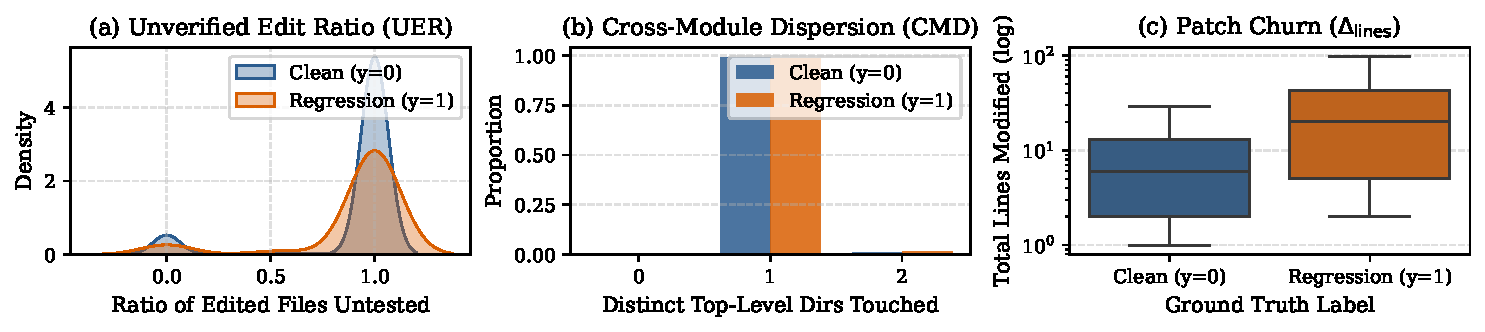
\includegraphics[width=\textwidth]{figures/v3/eda.pdf}
\reportcaption{figure}{Fold-0 training feature contrasts. Verification-gap features show little class separation; patch churn is more informative.}{fig:eda}
\vspace{8pt}
\begin{center}\small\setlength{\tabcolsep}{5pt}
\begin{tabular}{lcccc}
\toprule
Feature & \textbf{Clean ($y=0$)} & Regression ($y=1$) & $W$ & $D$ \\
\midrule
Unverified Edit Ratio & 1.0 [1.0, 1.0] & 1.0 [1.0, 1.0] & 0.03 & 0.01 \\
Cross-Module Dispersion & 1.0 [1.0, 1.0] & 1.0 [1.0, 1.0] & 0.10 & 0.01 \\
Post-Test Edits & 4.0 [3.0, 7.0] & 4.0 [2.0, 12.0] & 0.29 & 0.13 \\
Test Command Ratio & 0.06 [0.00, 0.12] & 0.04 [0.00, 0.11] & 0.20 & 0.11 \\
Total Edit Lines (Churn) & 6.0 [2.0, 13.0] & 20.0 [5.0, 43.0] & 1.41 & 0.38$^{***}$ \\
Files Modified & 1.0 [1.0, 1.0] & 1.0 [1.0, 1.0] & 0.51 & 0.10 \\
Hunks Modified & 1.0 [1.0, 2.0] & 2.0 [1.0, 3.0] & 0.56 & 0.24$^{**}$ \\
Terminal Tracebacks & 3.0 [2.0, 6.0] & 4.0 [2.0, 7.0] & 0.34 & 0.12 \\
Max Non-Zero Exit Streak & 1.0 [1.0, 2.0] & 1.0 [1.0, 2.0] & 0.11 & 0.05 \\
Repeated Commands & 0.00 [0.00, 0.00] & 0.00 [0.00, 0.00] & 0.13 & 0.02 \\
Tokens Received & 38931 [18612, 59169] & 46489 [21367, 67427] & 0.28 & 0.15 \\
Inference Cost (USD) & 0.42 [0.28, 0.65] & 0.59 [0.34, 0.85] & 0.50 & 0.23$^{**}$ \\
\bottomrule
\end{tabular}
\reportcaption{table}{Fold-0 training statistics: median [IQR], standardized Wasserstein distance $W$, and KS statistic $D$. Clean $n=1,540$; regression $n=61$. Stars denote unadjusted KS tests ($^{**}p<0.01$, $^{***}p<0.001$).}{tab:eda_stats}
\end{center}

\vspace{10pt}
\end{minipage}
}]
\section{Data and Ground Truth}
\label{sec:problem}
\paragraph{Category 4: Text / Logs.}
A detection unit is a completed agent run, its command/observation trace, and unified patch diff. Saved data cover seven model configurations: Claude-4.6-Opus, Claude-4.5-Opus, Claude-4.5-Sonnet, Gemini-3-Flash, Gemini-3-Pro, GPT-5.2, and DeepSeek-V3.2. Labels come from archived SWE-bench Verified evaluation reports.

Keep runs with zero F2P failures. Assign $y=1$ if P2P failures exceed zero, otherwise $y=0$. This gives $N=2,663$, $n_1=99$, $n_0=2,564$, and $\pi=3.72\%$. These are run counts, not independent issues. F2P refers to benchmark tests: it does not imply the agent authored or locally ran those exact tests.

\paragraph{Partition boundary.}
Five stratified group folds use \texttt{instance\_id} (439 issue groups). Train, validation, and test issue sets are disjoint within each fold. Repositories can occur in every split. This is issue-held-out evaluation; cross-project generalization is not established.

\section{Exploratory Analysis}
EDA uses Fold-0 training data only (1,540 clean and 61 regression runs). Regression patches have median churn 20 lines versus 6 for clean repairs. Churn's KS statistic is 0.38 ($p=3.2\times10^{-8}$). This is exploratory association, not a causal explanation. Both classes have median Unverified Edit Ratio and Cross-Module Dispersion 1.0.

H1 asks whether fusion improves AP over every individual channel. H2 asks whether variance equalization improves raw fusion. H3 asks whether contamination monotonically reduces performance. Section~\ref{sec:ablations} reports the observed outcomes.

\clearpage
\section{Method: CM-BAE}
\label{sec:method}
\subsection{Input Representation}
The structural channel has \textbf{12 dimensions}, including patch churn, file/hunk counts, test-command frequency, post-test edits, tracebacks, repeated commands, and resource usage. MiniLM provides 384 log dimensions; CodeBERT provides 768 diff dimensions. Frozen vectors summarize text patterns; they neither execute the patch nor prove semantic correctness.

Structural inputs are standardized on normal training runs. Channel weights use the mean feature variance from the same normals:
\begin{align}
v_m &= D_m^{-1}\sum_{j=1}^{D_m}\operatorname{Var}(x_{m,j}),\\
\alpha_m &= 1/\sqrt{\max(v_m,10^{-6})}.
\end{align}
Scaled channels are concatenated into $z\in\mathbb{R}^{1164}$. This equalizes average feature variance, not total channel energy; channel dimensions still differ.

\subsection{Normal-Reference Autoencoder}
The network widths are
\begin{equation}
1164\rightarrow256\rightarrow64\rightarrow256\rightarrow1164.
\end{equation}
Hidden layers use batch normalization and LeakyReLU. Dropout is 0.1 in the outer hidden layers. The 64-dimensional bottleneck provides about $18.2\times$ compression.

Only clean ($y=0$) training examples fit the autoencoder and preprocessing. Training uses Huber loss ($\delta=1$), Adam (learning rate $10^{-3}$, weight decay $10^{-5}$), cosine scheduling, 25 epochs, and batches of 64. For residual $r$,
\begin{equation}
\ell(r)=\begin{cases}r^2/2 & |r|\leq1,\\ |r|-1/2 & |r|>1.\end{cases}
\end{equation}
The objective limits large residuals' influence. A separate controlled comparison is needed to establish that this improves robustness here.

\subsection{Score and Attribution}
Each channel contributes its mean squared reconstruction error:
\begin{align}
s_m(x)&=D_m^{-1}\|z_m-\hat z_m\|_2^2,\\
s(x)&=s_{\mathrm{struct}}+s_{\mathrm{log}}+s_{\mathrm{patch}}.
\label{eq:additive}
\end{align}
Large error means this representation is difficult to reconstruct. It indicates atypicality, not a correctness verdict. Channel contributions explain the score, not a faulty line or the cause of a failed test.

\subsection{Labelled Calibration and Triage}
A logistic calibrator fits scores to \emph{labelled validation runs}, including regressions. Thus autoencoder fitting is normal-only, but the complete calibrated system is not wholly label-free.

The implementation scans 100 probability thresholds from 0.01 to 0.99 on validation data, maximizing
\begin{equation}
S(\tau)=1200\,\mathrm{TP}-30(\mathrm{TP}+\mathrm{FP}).
\end{equation}
Costs assume \$1,200 per escaped regression and \$30 per inspected candidate. If inspection prevents every reviewed regression, the probability break-even point is $30/1200=2.50\%$. These are scenario assumptions, not measured business outcomes.

\subsection{Reproducibility Boundary}
Saved features, partitions, benchmark summaries, and ablation results support the numbers. This revision rebuilds the report from those files; it does not repeat Docker evaluations, embedding extraction, or model training. Local specification checks verify selected consistency properties, not scientific validity or production readiness.

\clearpage
\twocolumn[{
\begin{minipage}{\textwidth}
\begin{center}\small\setlength{\tabcolsep}{5pt}
\begin{tabular}{lccccc}
\toprule
Method & AP $\uparrow$ & $F_2$ & ROC-AUC & Recall & FPR \\
\midrule
All-Normal & 0.037 $\pm$ 0.002 & 0.000 & 0.500 & 0.0\% & 0.0\% \\
3-Sigma Churn & 0.192 $\pm$ 0.140 & 0.175 & 0.712 & 16.5\% & 1.9\% \\
Unverified-Edit & 0.038 $\pm$ 0.004 & 0.162 & 0.504 & 90.8\% & 89.6\% \\
Inductive ECOD & 0.132 $\pm$ 0.054 & 0.190 & 0.687 & 20.3\% & 3.8\% \\
Isolation Forest & 0.141 $\pm$ 0.051 & 0.174 & 0.700 & 18.0\% & 3.4\% \\
Dual k-NN & 0.039 $\pm$ 0.006 & 0.029 & 0.470 & 3.1\% & 4.0\% \\
CM-BAE & 0.083 $\pm$ 0.028 & 0.145 & 0.596 & 82.9\% & 83.3\% \\
Supervised XGBoost & 0.096 $\pm$ 0.039 & 0.037 & 0.626 & 3.2\% & 0.5\% \\
Supervised MLP & 0.066 $\pm$ 0.031 & 0.120 & 0.551 & 15.2\% & 7.3\% \\
\bottomrule\end{tabular}
\reportcaption{table}{Five-fold benchmark (seed 42). AP is mean $\pm$ fold standard deviation. Threshold metrics use validation-selected operating points. CM-BAE is the proposed model, not the best performer.}{tab:main_benchmark}
\end{center}

\vspace{10pt}
\centering
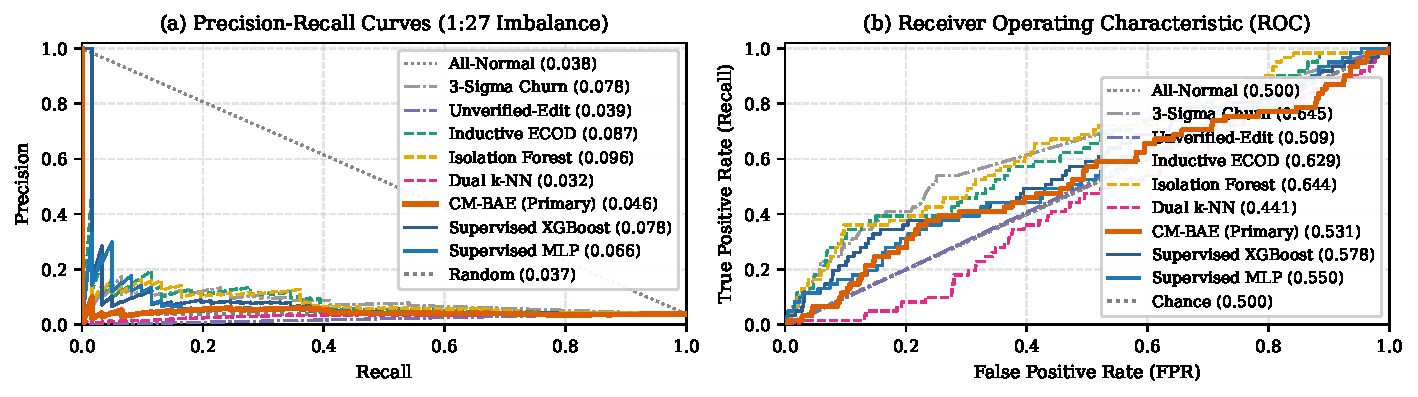
\includegraphics[width=0.94\textwidth]{figures/v3/pr_roc_curves.pdf}
\reportcaption{figure}{Diagnostic PR and ROC curves from the figure script's two-fold subset. These are illustrative; Table~\ref{tab:main_benchmark} reports five-fold performance.}{fig:curves}
\vspace{12pt}
\end{minipage}
}]
\section{Experimental Setup and Results}
\label{sec:experiments}
\label{sec:results}
\paragraph{Nine competitors.}
Tier 1 contains all-normal, patch churn, and an unverified-edit heuristic. Tier 2 contains ECOD, Isolation Forest, dual embedding $k$-NN, and CM-BAE. Tier 3 contains labelled XGBoost and multimodal MLP. Supervised models are reference competitors, not guaranteed upper bounds. Shared saved folds support comparisons.

\paragraph{Metrics.}
``PR-AUC'' denotes average precision (AP), not trapezoidal integration. Table values are means and standard deviations across seed-42 folds. Recall, FPR, and $F_2$ use validation-selected operating points. Ranking quality and threshold utility answer different questions.

\paragraph{Above prevalence, below strong controls.}
CM-BAE's fold AP is $0.0827\pm0.0281$. Its 25 seed-fold runs have mean $0.0827$ and standard deviation $0.0282$. This is $2.2\times$ prevalence. However, churn (0.192), Isolation Forest (0.141), ECOD (0.132), and XGBoost (0.096) score higher. CM-BAE exceeds dual $k$-NN and MLP, not all conventional or supervised methods.

\paragraph{Statistical scope.}
The saved paired test against all-normal fold AP gives $p=0.0336$ from five seed-42 fold pairs. This is exploratory and unadjusted: overlapping training sets and multiple comparisons limit a confirmatory interpretation. It does not establish superiority over the strongest control. Extra seeds do not create independent test issues.

\paragraph{Excessive review burden.}
The cost-selected CM-BAE threshold yields 82.9\% recall and 83.3\% FPR; mean balanced accuracy is about 0.498. Several folds flag every clean candidate. These results do not support low-noise automatic blocking, automatic release, or a guarantee that regressions cannot escape.

\clearpage
\twocolumn[{
\begin{minipage}{\textwidth}
\begin{center}\small\setlength{\tabcolsep}{5pt}
\begin{tabular}{lcc}
\toprule
Variant & AP $\uparrow$ & $F_2$ $\uparrow$ \\
\midrule
Full (Struct+Log+Patch+VarEq) & 0.083 $\pm$ 0.028 & 0.145 \\
Raw Fusion (w/o VarEq) & 0.123 $\pm$ 0.043 & 0.200 \\
Log-Only (MiniLM 384-D) & 0.044 $\pm$ 0.004 & 0.165 \\
Patch-Only (CodeBERT 768-D) & 0.048 $\pm$ 0.013 & 0.161 \\
Struct-Only (R0-struct 12-D) & 0.133 $\pm$ 0.048 & 0.148 \\
\bottomrule\end{tabular}
\reportcaption{table}{Saved modality ablations. Structural-only and raw fusion outperform the full equalized model.}{tab:ablation}
\end{center}

\vspace{12pt}
\centering
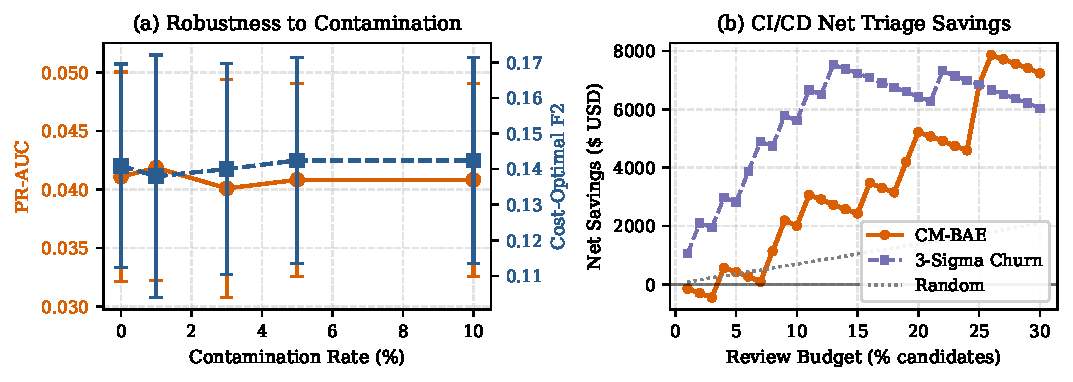
\includegraphics[width=0.9\textwidth,height=2.6in,keepaspectratio]{figures/v3/tradeoffs.pdf}
\reportcaption{figure}{Exploratory contamination and cost diagnostics. The cost curve uses Fold-0 test candidates and assumed costs; it is not a deployment savings measurement.}{fig:tradeoffs}
\vspace{12pt}
\end{minipage}
}]
\section{Ablations and Economic Limits}
\label{sec:ablations}
\paragraph{H1 is unsupported.}
Structural-only AP is 0.133, exceeding full fusion at 0.083. Log-only (0.044) and patch-only (0.048) are weak individually. These results do not establish semantic-channel gains. Additive attribution describes scores, but does not compensate for lower predictive performance.

\paragraph{H2 is unsupported.}
Raw fusion achieves AP 0.123 and $F_2$ 0.200, both higher than the equalized model. This contradicts a claim that equalization improves detection here. Altering channel contributions is a different outcome from improving screening.

\paragraph{H3 is unsupported.}
Contamination AP at 0\%, 1\%, 3\%, 5\%, and 10\% is 0.0411, 0.0419, 0.0401, 0.0408, and 0.0408. The trend is nearly flat and nonmonotonic. Its clean endpoint differs from the main AP of 0.0827. Treat it as a separate diagnostic with unresolved comparability, not proof of Huber robustness.

\paragraph{Cost sensitivity, not realized savings.}
The saved Fold-0 study reports \$6,840 at a 25\% review budget and \$7,230 at 30\%, relative to reviewing none under the assumed costs. At 1--3\% budgets the modeled savings are negative. Churn outperforms CM-BAE over many budgets. These results do not establish uniformly positive returns or \$13,800 saved per 1,000 PRs.

\paragraph{The review-all alternative matters.}
At prevalence 3.72\%, no review has assumed cost about \$44,611 per 1,000 candidates. Reviewing everything costs \$30,000 if inspection catches every regression. That policy already saves modeled cost without a ranking model. Value claims must compare with this option, capacity constraints, imperfect inspection, and measured engineering costs.

\paragraph{Practical implication.}
A usable detector must improve precision and residual risk at workloads engineers can sustain. Future evaluation needs repository-held-out or genuinely prospective data before supporting deployment decisions.

\clearpage
\twocolumn[{
\begin{minipage}{\textwidth}
\centering
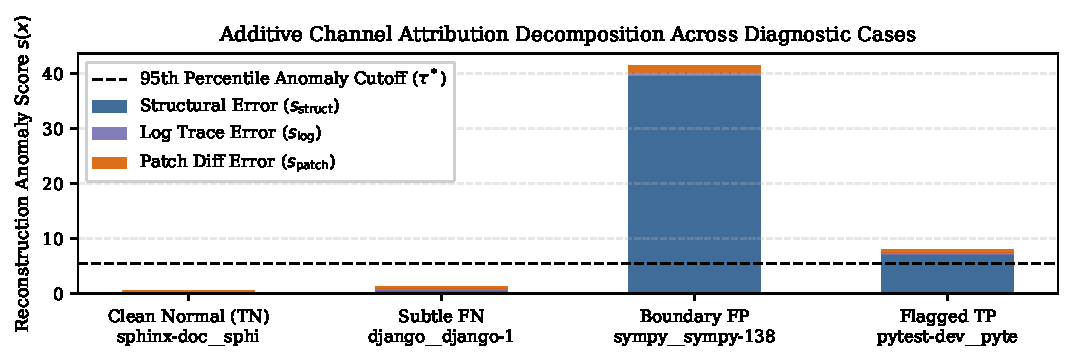
\includegraphics[width=0.85\textwidth,height=2.05in,keepaspectratio]{figures/v3/interpretability.pdf}
\reportcaption{figure}{Channel contributions for diagnostic cases. The dashed raw-score percentile is descriptive, not the validation-selected probability threshold used for TP/FP/FN/TN labels.}{fig:interp}
\vspace{12pt}
\end{minipage}
}]
\section{Error Analysis and Limitations}
\label{sec:error}
\paragraph{Diagnostic cases.}
Saved examples include a flagged regression on \texttt{pytest-6197} ($s=8.001$), a clean high-churn patch on \texttt{sympy-13878} incorrectly flagged ($s=41.454$), a missed regression on \texttt{django-15561} ($s=1.260$), and a clean example on \texttt{sphinx-8551} ($s=0.579$). Structural error dominates the high-churn false positive. Low reconstruction error can coexist with regression.

Scores and labels support these outcomes. Assertions about semantic causes require inspecting patches and failing tests; automatically generated descriptions alone do not establish root causes.

\paragraph{Unverified Edit Gap is a proxy.}
The extractor estimates whether edited paths are associated with test commands in the trace. No matching command does not prove a file was untested: a suite can exercise files without naming them. Both classes have median Unverified Edit Ratio 1.0, and heuristic AP is approximately chance (0.038). A high aggregate rate cannot establish the cause of the 99 regressions or a universal weakness of frontier agents.

\begin{minipage}{\columnwidth}
\paragraph{Generalization limits.}
Issues are held out; repositories are not. Test coverage limits label quality, and candidate selection determines prevalence. The cost analysis is hypothetical and single-fold. No production deployment, external submission, or reviewer acceptance follows from passing local checks.
\end{minipage}

\section{Conclusion}
There are 99 benchmark regressions among 2,663 F2P-passing candidates, a defensible rare-event screening population. CM-BAE exceeds prevalence, but structural controls rank better, fusion hypotheses are unsupported, and false alarms are excessive. The contribution is an exploratory benchmark that makes the remaining obstacles to a practical merge gate explicit.

\section*{Contributions of Each Member}
\ifdefined\JUDGE
Identities are omitted in this review version. Individual contribution allocations remain pending team confirmation.
\else
\begin{center}
\small
\begin{tabular}{ll}
\toprule
Member & Student ID\\
\midrule
Tun-Chieh Yang & 315553010\\
Jia-Cheng Wu & 314554059\\
Min-Quan Wang & 315553008\\
Wei-Chia Chang & 315553011\\
Chun-Ting Hou & 315554022\\
\bottomrule
\end{tabular}
\end{center}
Individual allocations remain pending confirmation, consistent with the saved team record.
\fi

\section*{AI Usage Statement}
AI assistants supported scaffolding, drafting, and graphics. This revision used Codex to audit saved results and repair layout. Metrics come from saved experiment outputs, not synthetic substitutes. This rebuild did not independently repeat upstream benchmark executions. Authors remain responsible for sources, analyses, and submission requirements.
